\documentclass[12pt,a4paper]{article}
%数学宏包
\usepackage{amsmath	}
\usepackage{amsbsy}
\usepackage{mathtools}
\usepackage{amssymb}
\usepackage{amsthm}
\usepackage{thmtools}
%图片
\usepackage{ graphicx}
%中文
\usepackage{ctex}
%页面设置
\usepackage{geometry}
\geometry{left=2cm,right=2cm,top=2cm,bottom=2cm}
% 标题格式设置
\usepackage{titlesec}
\usepackage{titletoc}
\titleformat{\section}{\Large\bfseries}{\thesection}{1em}{}
\titleformat{\subsection}{\large\bfseries}{\thesubsection}{1em}{}

\renewcommand{\(}{\left(}
\renewcommand{\)}{\right)}
\newcommand{\lra}{\Leftrightarrow}

\begin{document}\twocolumn
$$g(x)=-1-x+ \ln{x}+t$$
$$g \(x_1\)=g\(x_2\)=0$$
证$$x_1+x_2>t$$
证:
%插图
\begin{figure*}[b]
	\centering
	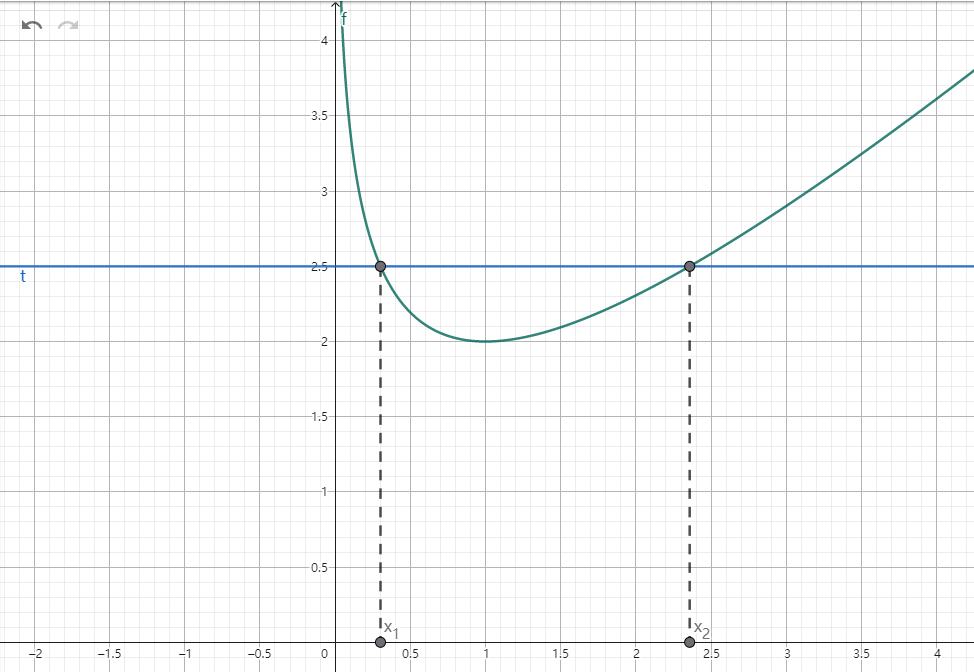
\includegraphics[height=8cm]{2}
	\caption{$y=x-\ln{x}+1$}{ $y=t$}
   
   \label{fig:1}
\end{figure*}


\begin{align*}
&g\(x\)=0\\
&\lra -1-x+ \ln{x}+t=0\\
&\lra x+1-\ln{x}=t
\end{align*}

如图1

易得$t>2$,{}不妨设$0<x_1<1<x_2$

\begin{equation*}
\begin{split}
\ & x_1+x_2>t\\
\lra & x_1+x_2>x_1+1- \ln{x_1}\\
\lra & x_2+ \ln{x_1}>{}1
\end{split}
\end{equation*}

设$$x_1=x_1 \left( t\right),x_2=x_2 \left( t\right)$$
$$h\(t\)=x_2+ \ln{x_1}$$
则只需证$$h\(t\)>1$$


\begin{equation} \label{a1}
\begin{split}
\ & g\(x_1\)=-1-x_1+ \ln{x_1}+t=0\\
 \ & g\(x_2\)=-1-x_2+ \ln{x_2}+t=0
\end{split}
\end{equation}

即
\begin{equation} \label{a2}
\begin{split}
\ & t=1+x_1- \ln{x_1}\\
\ & t=1+x_2- \ln{x_2}
\end{split}
\end{equation}

两侧对$t$求导
\begin{equation} \label{a3}
\begin{split}
\ & 1= \(   1- \frac{1}{x_1} \)x_1'\(t\)\\
\ & 1= \(   1- \frac{1}{x_2} \)x_2'\(t\)
\end{split}
\end{equation}

\begin{equation} \label{a4}
\begin{split}
\ & x_1'\(t\)= \frac{1}{1- \frac{1}{x_1} }=\frac{x_1}{x_1-1}\\
\ & x_2'\(t\)= \frac{1}{1- \frac{1}{x_2} }=\frac{x_2}{x_2-1}
\end{split}
\end{equation}

$$h\(t\)=x_2+ \ln{x_1}$$

对$t$求导
 
\begin{align}\label{a5}
h'\(t\)=& x_2'\(t\)+ \frac{x_1'\(t\)}{x_1} \notag \\
=& \frac{x_2}{x_2-1}+ \frac{\frac{x_1}{x_1-1}}{x_1} \notag\\
=&\frac{x_2}{x_2-1}+\frac{1}{x_1-1}\notag\\
=&\frac{x_1x_2-1}{\( x_1-1\)\( x_2-1\)}
\end{align}


已得$x_1<1{}, _2>1$,下证明{ }$x_1x_2{ }<{ }1$

\begin{align*}
\begin{cases}
t=1+x_1- \ln{x_1}\\
t=1+x_2- \ln{x_2}
\end{cases}
\end{align*}

上式减下式得

$$x_2-x_1 = \ln{x_2}-\ln{x_1}=\ln{\frac{x_2}{x_1}}$$

设$p=  \frac{x_2}{x_1}$,{ }$p>1$

\begin{align*}
\begin{cases}
x_2-x_1 =\ln{p} \\
p= \quad \frac{x_2}{x_1}
\end{cases}
\end{align*}

得
\begin{align*}
\begin{cases}
x_1=\quad \frac{p}{p-1} \ln{p}\\
x_2=\quad \frac{1}{p-1} \ln{p}
\end{cases}
\end{align*}


\begin{equation} \label{a6}
\begin{split}
x_1x_2=&\frac{p}{\(p-1\)^2} \ln^2{p}\\
=& \( \frac{ \sqrt{p}}{p-1} \ln{p}\)^2
\end{split}
\end{equation}

下证$\frac{ \sqrt{p}}{p-1} \ln{p} < 1$

\begin{equation} \label{a7}
\begin{split}
& \frac{ \sqrt{p}}{p-1} \ln{p} < 1\\
& \lra \ln{p}<\frac{p-1}{ \sqrt{p}}\\
& \text{设} q=\sqrt{p},\quad q>1\\
& \lra 2\ln{q} <\frac{q^2-1}{q}\\
& \lra 2\ln{q}-\frac{q^2-1}{q}<0
\end{split}
\end{equation}
设$m \(q \)= 2\ln{q}-\frac{q^2-1}{q}$
	
	\begin{align*}
	m' \( q \)&=2\frac{1}{q}-1-\frac{1}{q^2}\\
	&=\frac{2q-q^2-1}{q^2}\\
	&=-\frac{\(q-1\)^2}{q^2} { }<0
	\end{align*}
\begin{equation*}
\begin{gathered}
 \therefore m\(q\) \text{在} \(2,+\infty \){ }\downarrow\\
 \because q \to 2,m\(q\) \to 0\\
 \therefore q>0,{ }m\(q\)<0\\
 \therefore  \frac{ \sqrt{p}}{p-1} \ln{p} < 1\\
 \text{由} \(\ref{a6}\),{ }x_1x_2<1
\end{gathered}
\end{equation*}
\begin{align*}
&\text{由}\(\ref{a5}\),{ }h'\(t\)=\frac{x_1x_2-1}{\( x_1-1\)\( x_2-1\)}\\
&\because x_1<1,{  }x_2>1,{ }x_1x_2<1\\
&\therefore h'\(t\)>0\\
&h\(t\) \text{在} \(2,+\infty\) \uparrow \\
&\text{当}t \to2\\
&{ }x_1\to1,{ }x_1\to1,{ }\ln{x_1}\to0\\
&h\(t\)=x_2+ \ln{x_1}\to1\\
&\therefore t>2,h\(t\)>1\\
&\text{即证}
\end{align*}


\end{document}
